{\color{indiagreen}\subsection{Vrtenje tuljave v magnetnem polju}}
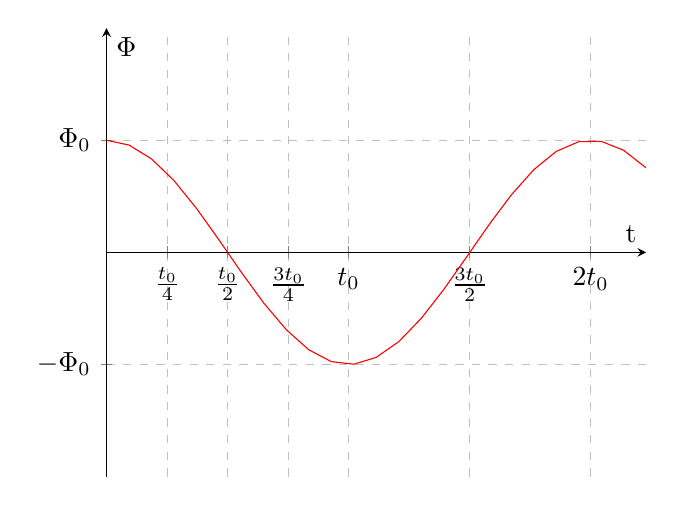
\begin{tikzpicture}
	\begin{axis}[
	    xlabel={t},
	    ylabel={$\Phi$},
	    xmin=0, xmax=7,
	    ymin=-2, ymax=2,
	    xtick={0,0.79, 1.57, 2.36, 3.14, 4.71, 6.28},
	    ytick={-1,0,1},
	    xticklabels={0,$\frac{t_0}{4}$, $\frac{t_0}{2}$, $\frac{3t_0}{4}$, $t_0$, $\frac{3t_0}{2}$, $2t_0$},
	    yticklabels={$-\Phi_0$, 0, $\Phi_0$},
	    ymajorgrids=true,
	    xmajorgrids=true,
	    grid style=dashed,
	    axis lines=middle,
	]
	\addplot[domain=0:7,red] {cos(deg(x))};
	\end{axis}
\end{tikzpicture}\\
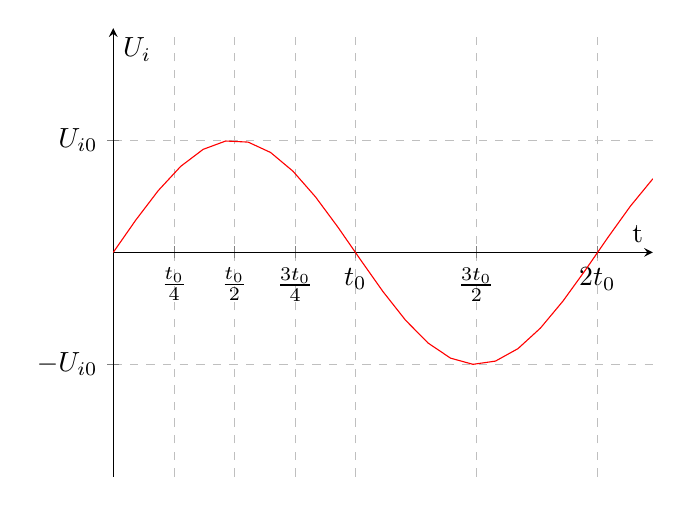
\begin{tikzpicture}
	\begin{axis}[
	    xlabel={t},
	    ylabel={$U_i$},
	    xmin=0, xmax=7,
	    ymin=-2, ymax=2,
	    xtick={0,0.79, 1.57, 2.36, 3.14, 4.71, 6.28},
	    ytick={-1,0,1},
	    xticklabels={0,$\frac{t_0}{4}$, $\frac{t_0}{2}$, $\frac{3t_0}{4}$, $t_0$, $\frac{3t_0}{2}$, $2t_0$},
	    yticklabels={$-U_{i0}$, 0, $U_{i0}$},
	    ymajorgrids=true,
	    xmajorgrids=true,
	    grid style=dashed,
	    axis lines=middle,
	]
	\addplot[domain=0:7,red] {sin(deg(x))};
	\end{axis}
\end{tikzpicture}\\
%\begin{center}
%	\includegraphics[width=15cm, height=15cm,keepaspectratio=true]{VrtenjeTuljaveVMagPol.png}
%\end{center}
\begin{align*}
	\varphi = \omega t &\rightarrow \omega = 2\pi\nu\\
	{\color{bostonuniversityred}\Phi} &= {\color{bostonuniversityred}\Phi_0 \cos(\omega t)}\\ 
	\Phi_0 &= NBS\\
	U_i &= \frac{\Delta \Phi}{\Delta t}\\
	U_i &= U_{i0} \sin(\omega t)
	\Phi &= \Phi_0 \cos(\omega t)\\
	{\color{bostonuniversityred}\Phi^{'}} = {\color{bostonuniversityred}U_i = \omega \Phi_0 \sin(\omega t)} &\dots \text{odvod od $\Phi$ je $U_i$ ker je odvod od cosinsa sinus in $\omega \Phi_0 = U_{i0}$}\\
	{\color{bostonuniversityred}U_{i0}} &= {\color{bostonuniversityred}\omega NBS}\\
\end{align*}
Ko vrtiumo tuljavo v magnetnem polju, dobimo izmenično napetost.\\